% !TEX TS-program = pdflatex
% !TEX encoding = UTF-8 Unicode
\documentclass[border=0mm]{standalone}
% packages
\usepackage{tikz}
\usetikzlibrary{patterns}
\usepackage{amsmath,amssymb}
\usepackage{bm}
\usepackage{pgfplots}
\pgfplotsset{compat=1.15}
% start document
\begin{document}
% generated by ROOT (CERN)
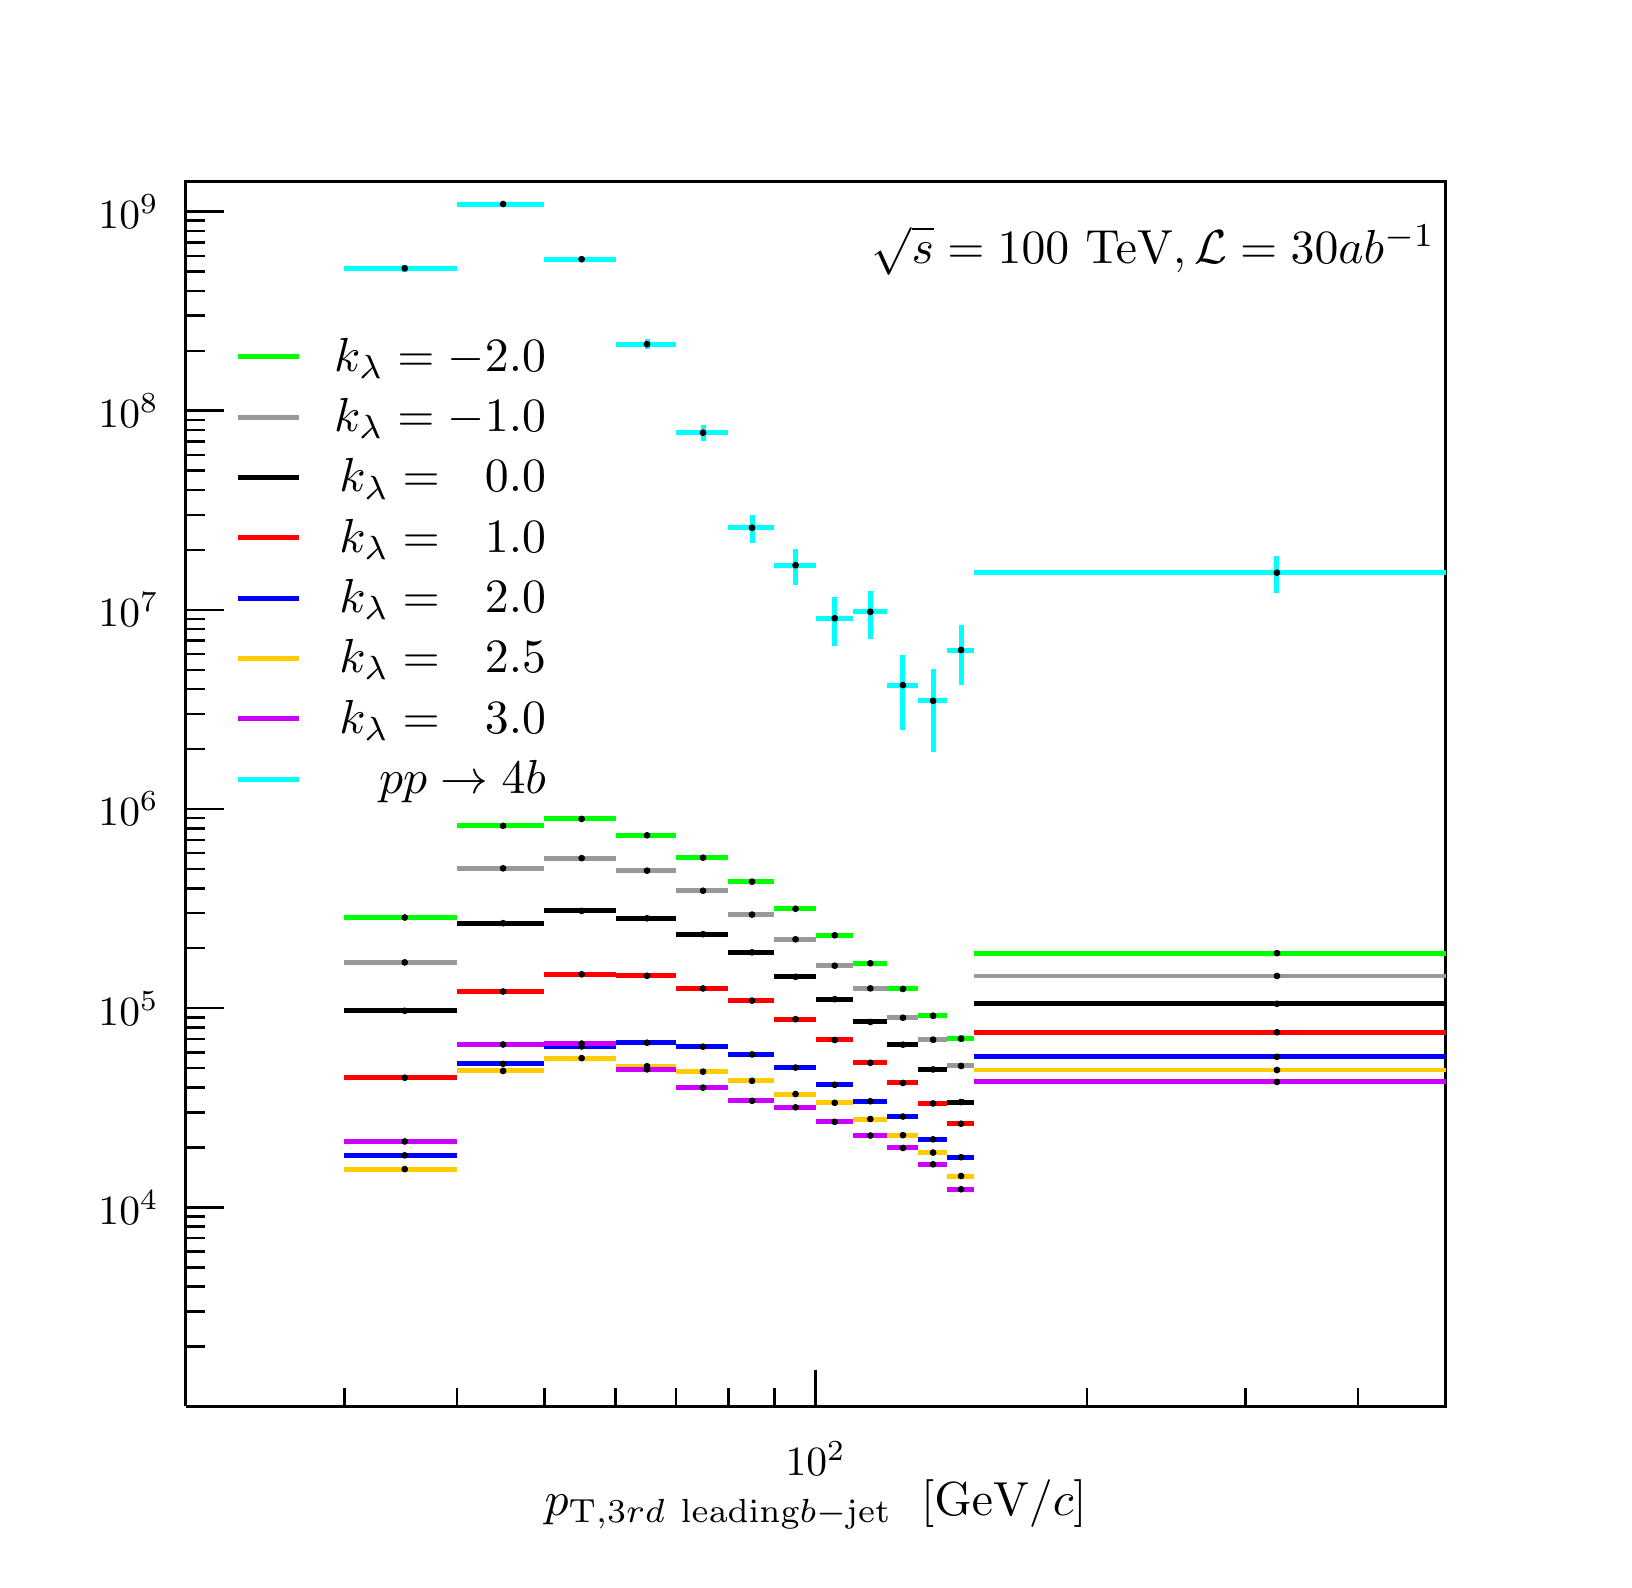
\begin{tikzpicture}
\pgfdeclareplotmark{cross} {
\pgfpathmoveto{\pgfpoint{-0.3\pgfplotmarksize}{\pgfplotmarksize}}
\pgfpathlineto{\pgfpoint{+0.3\pgfplotmarksize}{\pgfplotmarksize}}
\pgfpathlineto{\pgfpoint{+0.3\pgfplotmarksize}{0.3\pgfplotmarksize}}
\pgfpathlineto{\pgfpoint{+1\pgfplotmarksize}{0.3\pgfplotmarksize}}
\pgfpathlineto{\pgfpoint{+1\pgfplotmarksize}{-0.3\pgfplotmarksize}}
\pgfpathlineto{\pgfpoint{+0.3\pgfplotmarksize}{-0.3\pgfplotmarksize}}
\pgfpathlineto{\pgfpoint{+0.3\pgfplotmarksize}{-1.\pgfplotmarksize}}
\pgfpathlineto{\pgfpoint{-0.3\pgfplotmarksize}{-1.\pgfplotmarksize}}
\pgfpathlineto{\pgfpoint{-0.3\pgfplotmarksize}{-0.3\pgfplotmarksize}}
\pgfpathlineto{\pgfpoint{-1.\pgfplotmarksize}{-0.3\pgfplotmarksize}}
\pgfpathlineto{\pgfpoint{-1.\pgfplotmarksize}{0.3\pgfplotmarksize}}
\pgfpathlineto{\pgfpoint{-0.3\pgfplotmarksize}{0.3\pgfplotmarksize}}
\pgfpathclose
\pgfusepathqstroke
}
\pgfdeclareplotmark{cross*} {
\pgfpathmoveto{\pgfpoint{-0.3\pgfplotmarksize}{\pgfplotmarksize}}
\pgfpathlineto{\pgfpoint{+0.3\pgfplotmarksize}{\pgfplotmarksize}}
\pgfpathlineto{\pgfpoint{+0.3\pgfplotmarksize}{0.3\pgfplotmarksize}}
\pgfpathlineto{\pgfpoint{+1\pgfplotmarksize}{0.3\pgfplotmarksize}}
\pgfpathlineto{\pgfpoint{+1\pgfplotmarksize}{-0.3\pgfplotmarksize}}
\pgfpathlineto{\pgfpoint{+0.3\pgfplotmarksize}{-0.3\pgfplotmarksize}}
\pgfpathlineto{\pgfpoint{+0.3\pgfplotmarksize}{-1.\pgfplotmarksize}}
\pgfpathlineto{\pgfpoint{-0.3\pgfplotmarksize}{-1.\pgfplotmarksize}}
\pgfpathlineto{\pgfpoint{-0.3\pgfplotmarksize}{-0.3\pgfplotmarksize}}
\pgfpathlineto{\pgfpoint{-1.\pgfplotmarksize}{-0.3\pgfplotmarksize}}
\pgfpathlineto{\pgfpoint{-1.\pgfplotmarksize}{0.3\pgfplotmarksize}}
\pgfpathlineto{\pgfpoint{-0.3\pgfplotmarksize}{0.3\pgfplotmarksize}}
\pgfpathclose
\pgfusepathqfillstroke
}
\pgfdeclareplotmark{newstar} {
\pgfpathmoveto{\pgfqpoint{0pt}{\pgfplotmarksize}}
\pgfpathlineto{\pgfqpointpolar{44}{0.5\pgfplotmarksize}}
\pgfpathlineto{\pgfqpointpolar{18}{\pgfplotmarksize}}
\pgfpathlineto{\pgfqpointpolar{-20}{0.5\pgfplotmarksize}}
\pgfpathlineto{\pgfqpointpolar{-54}{\pgfplotmarksize}}
\pgfpathlineto{\pgfqpointpolar{-90}{0.5\pgfplotmarksize}}
\pgfpathlineto{\pgfqpointpolar{234}{\pgfplotmarksize}}
\pgfpathlineto{\pgfqpointpolar{198}{0.5\pgfplotmarksize}}
\pgfpathlineto{\pgfqpointpolar{162}{\pgfplotmarksize}}
\pgfpathlineto{\pgfqpointpolar{134}{0.5\pgfplotmarksize}}
\pgfpathclose
\pgfusepathqstroke
}
\pgfdeclareplotmark{newstar*} {
\pgfpathmoveto{\pgfqpoint{0pt}{\pgfplotmarksize}}
\pgfpathlineto{\pgfqpointpolar{44}{0.5\pgfplotmarksize}}
\pgfpathlineto{\pgfqpointpolar{18}{\pgfplotmarksize}}
\pgfpathlineto{\pgfqpointpolar{-20}{0.5\pgfplotmarksize}}
\pgfpathlineto{\pgfqpointpolar{-54}{\pgfplotmarksize}}
\pgfpathlineto{\pgfqpointpolar{-90}{0.5\pgfplotmarksize}}
\pgfpathlineto{\pgfqpointpolar{234}{\pgfplotmarksize}}
\pgfpathlineto{\pgfqpointpolar{198}{0.5\pgfplotmarksize}}
\pgfpathlineto{\pgfqpointpolar{162}{\pgfplotmarksize}}
\pgfpathlineto{\pgfqpointpolar{134}{0.5\pgfplotmarksize}}
\pgfpathclose
\pgfusepathqfillstroke
}
\definecolor{c}{rgb}{1,1,1};
\draw [color=c, fill=c] (0,0) rectangle (20,19.4486);
\draw [color=c, fill=c] (0,0) rectangle (20,19.4486);
\draw [color=c, fill=c] (2,1.94486) rectangle (18,17.5038);
\definecolor{c}{rgb}{0,0,0};
\draw [c,line width=0.9] (2,1.94486) -- (2,17.5038) -- (18,17.5038) -- (18,1.94486) -- (2,1.94486);
\definecolor{c}{rgb}{1,1,1};
\draw [color=c, fill=c] (2,1.94486) rectangle (18,17.5038);
\definecolor{c}{rgb}{0,0,0};
\draw [c,line width=0.9] (2,1.94486) -- (2,17.5038) -- (18,17.5038) -- (18,1.94486) -- (2,1.94486);
\definecolor{c}{rgb}{0,1,1};
\draw [c,line width=1.8] (4.78167,16.3584) -- (4.78167,16.3994);
\draw [c,line width=1.8] (4.78167,16.3994) -- (4.78167,16.439);
\draw [c,line width=1.8] (4.01544,16.3994) -- (4.78167,16.3994);
\draw [c,line width=1.8] (4.78167,16.3994) -- (5.44541,16.3994);
\definecolor{c}{rgb}{0,0,0};
\foreach \P in {(4.78167,16.3994)}{\draw[mark options={color=c,fill=c},mark size=2.402402pt,mark=*,mark size=1pt] plot coordinates {\P};}
\definecolor{c}{rgb}{0,1,1};
\draw [c,line width=1.8] (6.03087,17.1874) -- (6.03087,17.2156);
\draw [c,line width=1.8] (6.03087,17.2156) -- (6.03087,17.243);
\draw [c,line width=1.8] (5.44541,17.2156) -- (6.03087,17.2156);
\draw [c,line width=1.8] (6.03087,17.2156) -- (6.55459,17.2156);
\definecolor{c}{rgb}{0,0,0};
\foreach \P in {(6.03087,17.2156)}{\draw[mark options={color=c,fill=c},mark size=2.402402pt,mark=*,mark size=1pt] plot coordinates {\P};}
\definecolor{c}{rgb}{0,1,1};
\draw [c,line width=1.8] (7.02834,16.4755) -- (7.02834,16.5144);
\draw [c,line width=1.8] (7.02834,16.5144) -- (7.02834,16.552);
\draw [c,line width=1.8] (6.55459,16.5144) -- (7.02834,16.5144);
\draw [c,line width=1.8] (7.02834,16.5144) -- (7.46085,16.5144);
\definecolor{c}{rgb}{0,0,0};
\foreach \P in {(7.02834,16.5144)}{\draw[mark options={color=c,fill=c},mark size=2.402402pt,mark=*,mark size=1pt] plot coordinates {\P};}
\definecolor{c}{rgb}{0,1,1};
\draw [c,line width=1.8] (7.85872,15.3714) -- (7.85872,15.4357);
\draw [c,line width=1.8] (7.85872,15.4357) -- (7.85872,15.4965);
\draw [c,line width=1.8] (7.46085,15.4357) -- (7.85872,15.4357);
\draw [c,line width=1.8] (7.85872,15.4357) -- (8.22708,15.4357);
\definecolor{c}{rgb}{0,0,0};
\foreach \P in {(7.85872,15.4357)}{\draw[mark options={color=c,fill=c},mark size=2.402402pt,mark=*,mark size=1pt] plot coordinates {\P};}
\definecolor{c}{rgb}{0,1,1};
\draw [c,line width=1.8] (8.57002,14.2016) -- (8.57002,14.3112);
\draw [c,line width=1.8] (8.57002,14.3112) -- (8.57002,14.4108);
\draw [c,line width=1.8] (8.22708,14.3112) -- (8.57002,14.3112);
\draw [c,line width=1.8] (8.57002,14.3112) -- (8.89083,14.3112);
\definecolor{c}{rgb}{0,0,0};
\foreach \P in {(8.57002,14.3112)}{\draw[mark options={color=c,fill=c},mark size=2.402402pt,mark=*,mark size=1pt] plot coordinates {\P};}
\definecolor{c}{rgb}{0,1,1};
\draw [c,line width=1.8] (9.19217,12.9072) -- (9.19217,13.1045);
\draw [c,line width=1.8] (9.19217,13.1045) -- (9.19217,13.2716);
\draw [c,line width=1.8] (8.89083,13.1045) -- (9.19217,13.1045);
\draw [c,line width=1.8] (9.19217,13.1045) -- (9.47629,13.1045);
\definecolor{c}{rgb}{0,0,0};
\foreach \P in {(9.19217,13.1045)}{\draw[mark options={color=c,fill=c},mark size=2.402402pt,mark=*,mark size=1pt] plot coordinates {\P};}
\definecolor{c}{rgb}{0,1,1};
\draw [c,line width=1.8] (9.74504,12.3782) -- (9.74504,12.629);
\draw [c,line width=1.8] (9.74504,12.629) -- (9.74504,12.833);
\draw [c,line width=1.8] (9.47629,12.629) -- (9.74504,12.629);
\draw [c,line width=1.8] (9.74504,12.629) -- (10,12.629);
\definecolor{c}{rgb}{0,0,0};
\foreach \P in {(9.74504,12.629)}{\draw[mark options={color=c,fill=c},mark size=2.402402pt,mark=*,mark size=1pt] plot coordinates {\P};}
\definecolor{c}{rgb}{0,1,1};
\draw [c,line width=1.8] (10.2425,11.5988) -- (10.2425,11.9556);
\draw [c,line width=1.8] (10.2425,11.9556) -- (10.2425,12.2244);
\draw [c,line width=1.8] (10,11.9556) -- (10.2425,11.9556);
\draw [c,line width=1.8] (10.2425,11.9556) -- (10.4738,11.9556);
\definecolor{c}{rgb}{0,0,0};
\foreach \P in {(10.2425,11.9556)}{\draw[mark options={color=c,fill=c},mark size=2.402402pt,mark=*,mark size=1pt] plot coordinates {\P};}
\definecolor{c}{rgb}{0,1,1};
\draw [c,line width=1.8] (10.6947,11.6954) -- (10.6947,12.037);
\draw [c,line width=1.8] (10.6947,12.037) -- (10.6947,12.2971);
\draw [c,line width=1.8] (10.4738,12.037) -- (10.6947,12.037);
\draw [c,line width=1.8] (10.6947,12.037) -- (10.9063,12.037);
\definecolor{c}{rgb}{0,0,0};
\foreach \P in {(10.6947,12.037)}{\draw[mark options={color=c,fill=c},mark size=2.402402pt,mark=*,mark size=1pt] plot coordinates {\P};}
\definecolor{c}{rgb}{0,1,1};
\draw [c,line width=1.8] (11.1092,10.53) -- (11.1092,11.1063);
\draw [c,line width=1.8] (11.1092,11.1063) -- (11.1092,11.4823);
\draw [c,line width=1.8] (10.9063,11.1063) -- (11.1092,11.1063);
\draw [c,line width=1.8] (11.1092,11.1063) -- (11.3041,11.1063);
\definecolor{c}{rgb}{0,0,0};
\foreach \P in {(11.1092,11.1063)}{\draw[mark options={color=c,fill=c},mark size=2.402402pt,mark=*,mark size=1pt] plot coordinates {\P};}
\definecolor{c}{rgb}{0,1,1};
\draw [c,line width=1.8] (11.4917,10.2549) -- (11.4917,10.906);
\draw [c,line width=1.8] (11.4917,10.906) -- (11.4917,11.312);
\draw [c,line width=1.8] (11.3041,10.906) -- (11.4917,10.906);
\draw [c,line width=1.8] (11.4917,10.906) -- (11.6725,10.906);
\definecolor{c}{rgb}{0,0,0};
\foreach \P in {(11.4917,10.906)}{\draw[mark options={color=c,fill=c},mark size=2.402402pt,mark=*,mark size=1pt] plot coordinates {\P};}
\definecolor{c}{rgb}{0,1,1};
\draw [c,line width=1.8] (11.8469,11.1063) -- (11.8469,11.5517);
\draw [c,line width=1.8] (11.8469,11.5517) -- (11.8469,11.8677);
\draw [c,line width=1.8] (11.6725,11.5517) -- (11.8469,11.5517);
\draw [c,line width=1.8] (11.8469,11.5517) -- (12.0154,11.5517);
\definecolor{c}{rgb}{0,0,0};
\foreach \P in {(11.8469,11.5517)}{\draw[mark options={color=c,fill=c},mark size=2.402402pt,mark=*,mark size=1pt] plot coordinates {\P};}
\definecolor{c}{rgb}{0,1,1};
\draw [c,line width=1.8] (15.8587,12.2701) -- (15.8587,12.5334);
\draw [c,line width=1.8] (15.8587,12.5334) -- (15.8587,12.7457);
\draw [c,line width=1.8] (12.0154,12.5334) -- (15.8587,12.5334);
\draw [c,line width=1.8] (15.8587,12.5334) -- (18,12.5334);
\definecolor{c}{rgb}{0,0,0};
\foreach \P in {(15.8587,12.5334)}{\draw[mark options={color=c,fill=c},mark size=2.402402pt,mark=*,mark size=1pt] plot coordinates {\P};}
\draw [c,line width=0.9] (2,1.94486) -- (18,1.94486);
\draw [c,line width=0.9] (4.01543,2.17825) -- (4.01543,1.94486);
\draw [c,line width=0.9] (5.4454,2.17825) -- (5.4454,1.94486);
\draw [c,line width=0.9] (6.55458,2.17825) -- (6.55458,1.94486);
\draw [c,line width=0.9] (7.46084,2.17825) -- (7.46084,1.94486);
\draw [c,line width=0.9] (8.22708,2.17825) -- (8.22708,1.94486);
\draw [c,line width=0.9] (8.89082,2.17825) -- (8.89082,1.94486);
\draw [c,line width=0.9] (9.47628,2.17825) -- (9.47628,1.94486);
\draw [c,line width=0.9] (9.99999,2.41163) -- (9.99999,1.94486);
\draw [anchor=base] (9.99999,1.06481) node[scale=1.50291, color=c, rotate=0]{$10^{2}$};
\draw [c,line width=0.9] (13.4454,2.17825) -- (13.4454,1.94486);
\draw [c,line width=0.9] (15.4608,2.17825) -- (15.4608,1.94486);
\draw [c,line width=0.9] (16.8908,2.17825) -- (16.8908,1.94486);
\draw [c,line width=0.9] (18,2.17825) -- (18,1.94486);
\draw (10,0.700151) node[scale=1.72557, color=c, rotate=0]{$ p_{\text{T}, 3rd ~\text{leading} b-\text{jet~}} ~[\text{GeV}/c]$};
\draw [c,line width=0.9] (2,1.94486) -- (2,17.5038);
\draw [c,line width=0.9] (2.24,2.70622) -- (2,2.70622);
\draw [c,line width=0.9] (2.24,3.15158) -- (2,3.15158);
\draw [c,line width=0.9] (2.24,3.46757) -- (2,3.46757);
\draw [c,line width=0.9] (2.24,3.71267) -- (2,3.71267);
\draw [c,line width=0.9] (2.24,3.91294) -- (2,3.91294);
\draw [c,line width=0.9] (2.24,4.08225) -- (2,4.08225);
\draw [c,line width=0.9] (2.24,4.22893) -- (2,4.22893);
\draw [c,line width=0.9] (2.24,4.3583) -- (2,4.3583);
\draw [c,line width=0.9] (2.48,4.47403) -- (2,4.47403);
\draw [anchor= east] (1.844,4.47403) node[scale=1.50291, color=c, rotate=0]{$10^{4}$};
\draw [c,line width=0.9] (2.24,5.23538) -- (2,5.23538);
\draw [c,line width=0.9] (2.24,5.68075) -- (2,5.68075);
\draw [c,line width=0.9] (2.24,5.99674) -- (2,5.99674);
\draw [c,line width=0.9] (2.24,6.24184) -- (2,6.24184);
\draw [c,line width=0.9] (2.24,6.4421) -- (2,6.4421);
\draw [c,line width=0.9] (2.24,6.61142) -- (2,6.61142);
\draw [c,line width=0.9] (2.24,6.75809) -- (2,6.75809);
\draw [c,line width=0.9] (2.24,6.88747) -- (2,6.88747);
\draw [c,line width=0.9] (2.48,7.0032) -- (2,7.0032);
\draw [anchor= east] (1.844,7.0032) node[scale=1.50291, color=c, rotate=0]{$10^{5}$};
\draw [c,line width=0.9] (2.24,7.76455) -- (2,7.76455);
\draw [c,line width=0.9] (2.24,8.20992) -- (2,8.20992);
\draw [c,line width=0.9] (2.24,8.52591) -- (2,8.52591);
\draw [c,line width=0.9] (2.24,8.77101) -- (2,8.77101);
\draw [c,line width=0.9] (2.24,8.97127) -- (2,8.97127);
\draw [c,line width=0.9] (2.24,9.14059) -- (2,9.14059);
\draw [c,line width=0.9] (2.24,9.28726) -- (2,9.28726);
\draw [c,line width=0.9] (2.24,9.41664) -- (2,9.41664);
\draw [c,line width=0.9] (2.48,9.53236) -- (2,9.53236);
\draw [anchor= east] (1.844,9.53236) node[scale=1.50291, color=c, rotate=0]{$10^{6}$};
\draw [c,line width=0.9] (2.24,10.2937) -- (2,10.2937);
\draw [c,line width=0.9] (2.24,10.7391) -- (2,10.7391);
\draw [c,line width=0.9] (2.24,11.0551) -- (2,11.0551);
\draw [c,line width=0.9] (2.24,11.3002) -- (2,11.3002);
\draw [c,line width=0.9] (2.24,11.5004) -- (2,11.5004);
\draw [c,line width=0.9] (2.24,11.6698) -- (2,11.6698);
\draw [c,line width=0.9] (2.24,11.8164) -- (2,11.8164);
\draw [c,line width=0.9] (2.24,11.9458) -- (2,11.9458);
\draw [c,line width=0.9] (2.48,12.0615) -- (2,12.0615);
\draw [anchor= east] (1.844,12.0615) node[scale=1.50291, color=c, rotate=0]{$10^{7}$};
\draw [c,line width=0.9] (2.24,12.8229) -- (2,12.8229);
\draw [c,line width=0.9] (2.24,13.2683) -- (2,13.2683);
\draw [c,line width=0.9] (2.24,13.5842) -- (2,13.5842);
\draw [c,line width=0.9] (2.24,13.8293) -- (2,13.8293);
\draw [c,line width=0.9] (2.24,14.0296) -- (2,14.0296);
\draw [c,line width=0.9] (2.24,14.1989) -- (2,14.1989);
\draw [c,line width=0.9] (2.24,14.3456) -- (2,14.3456);
\draw [c,line width=0.9] (2.24,14.475) -- (2,14.475);
\draw [c,line width=0.9] (2.48,14.5907) -- (2,14.5907);
\draw [anchor= east] (1.844,14.5907) node[scale=1.50291, color=c, rotate=0]{$10^{8}$};
\draw [c,line width=0.9] (2.24,15.3521) -- (2,15.3521);
\draw [c,line width=0.9] (2.24,15.7974) -- (2,15.7974);
\draw [c,line width=0.9] (2.24,16.1134) -- (2,16.1134);
\draw [c,line width=0.9] (2.24,16.3585) -- (2,16.3585);
\draw [c,line width=0.9] (2.24,16.5588) -- (2,16.5588);
\draw [c,line width=0.9] (2.24,16.7281) -- (2,16.7281);
\draw [c,line width=0.9] (2.24,16.8748) -- (2,16.8748);
\draw [c,line width=0.9] (2.24,17.0041) -- (2,17.0041);
\draw [c,line width=0.9] (2.48,17.1199) -- (2,17.1199);
\draw [anchor= east] (1.844,17.1199) node[scale=1.50291, color=c, rotate=0]{$10^{9}$};
\definecolor{c}{rgb}{0,1,0};
\draw [c,line width=1.8] (4.78167,8.13152) -- (4.78167,8.15472);
\draw [c,line width=1.8] (4.78167,8.15472) -- (4.78167,8.17744);
\draw [c,line width=1.8] (4.01544,8.15472) -- (4.78167,8.15472);
\draw [c,line width=1.8] (4.78167,8.15472) -- (5.44541,8.15472);
\definecolor{c}{rgb}{0,0,0};
\foreach \P in {(4.78167,8.15472)}{\draw[mark options={color=c,fill=c},mark size=2.402402pt,mark=*,mark size=1pt] plot coordinates {\P};}
\definecolor{c}{rgb}{0,1,0};
\draw [c,line width=1.8] (6.03087,9.30564) -- (6.03087,9.31923);
\draw [c,line width=1.8] (6.03087,9.31923) -- (6.03087,9.33266);
\draw [c,line width=1.8] (5.44541,9.31923) -- (6.03087,9.31923);
\draw [c,line width=1.8] (6.03087,9.31923) -- (6.55459,9.31923);
\definecolor{c}{rgb}{0,0,0};
\foreach \P in {(6.03087,9.31923)}{\draw[mark options={color=c,fill=c},mark size=2.402402pt,mark=*,mark size=1pt] plot coordinates {\P};}
\definecolor{c}{rgb}{0,1,0};
\draw [c,line width=1.8] (7.02834,9.39364) -- (7.02834,9.4067);
\draw [c,line width=1.8] (7.02834,9.4067) -- (7.02834,9.41961);
\draw [c,line width=1.8] (6.55459,9.4067) -- (7.02834,9.4067);
\draw [c,line width=1.8] (7.02834,9.4067) -- (7.46085,9.4067);
\definecolor{c}{rgb}{0,0,0};
\foreach \P in {(7.02834,9.4067)}{\draw[mark options={color=c,fill=c},mark size=2.402402pt,mark=*,mark size=1pt] plot coordinates {\P};}
\definecolor{c}{rgb}{0,1,0};
\draw [c,line width=1.8] (7.85872,9.18416) -- (7.85872,9.19852);
\draw [c,line width=1.8] (7.85872,9.19852) -- (7.85872,9.2127);
\draw [c,line width=1.8] (7.46085,9.19852) -- (7.85872,9.19852);
\draw [c,line width=1.8] (7.85872,9.19852) -- (8.22708,9.19852);
\definecolor{c}{rgb}{0,0,0};
\foreach \P in {(7.85872,9.19852)}{\draw[mark options={color=c,fill=c},mark size=2.402402pt,mark=*,mark size=1pt] plot coordinates {\P};}
\definecolor{c}{rgb}{0,1,0};
\draw [c,line width=1.8] (8.57002,8.89827) -- (8.57002,8.91464);
\draw [c,line width=1.8] (8.57002,8.91464) -- (8.57002,8.93076);
\draw [c,line width=1.8] (8.22708,8.91464) -- (8.57002,8.91464);
\draw [c,line width=1.8] (8.57002,8.91464) -- (8.89083,8.91464);
\definecolor{c}{rgb}{0,0,0};
\foreach \P in {(8.57002,8.91464)}{\draw[mark options={color=c,fill=c},mark size=2.402402pt,mark=*,mark size=1pt] plot coordinates {\P};}
\definecolor{c}{rgb}{0,1,0};
\draw [c,line width=1.8] (9.19217,8.59146) -- (9.19217,8.61027);
\draw [c,line width=1.8] (9.19217,8.61027) -- (9.19217,8.62877);
\draw [c,line width=1.8] (8.89083,8.61027) -- (9.19217,8.61027);
\draw [c,line width=1.8] (9.19217,8.61027) -- (9.47629,8.61027);
\definecolor{c}{rgb}{0,0,0};
\foreach \P in {(9.19217,8.61027)}{\draw[mark options={color=c,fill=c},mark size=2.402402pt,mark=*,mark size=1pt] plot coordinates {\P};}
\definecolor{c}{rgb}{0,1,0};
\draw [c,line width=1.8] (9.74504,8.24345) -- (9.74504,8.2655);
\draw [c,line width=1.8] (9.74504,8.2655) -- (9.74504,8.28711);
\draw [c,line width=1.8] (9.47629,8.2655) -- (9.74504,8.2655);
\draw [c,line width=1.8] (9.74504,8.2655) -- (10,8.2655);
\definecolor{c}{rgb}{0,0,0};
\foreach \P in {(9.74504,8.2655)}{\draw[mark options={color=c,fill=c},mark size=2.402402pt,mark=*,mark size=1pt] plot coordinates {\P};}
\definecolor{c}{rgb}{0,1,0};
\draw [c,line width=1.8] (10.2425,7.9029) -- (10.2425,7.92864);
\draw [c,line width=1.8] (10.2425,7.92864) -- (10.2425,7.95379);
\draw [c,line width=1.8] (10,7.92864) -- (10.2425,7.92864);
\draw [c,line width=1.8] (10.2425,7.92864) -- (10.4738,7.92864);
\definecolor{c}{rgb}{0,0,0};
\foreach \P in {(10.2425,7.92864)}{\draw[mark options={color=c,fill=c},mark size=2.402402pt,mark=*,mark size=1pt] plot coordinates {\P};}
\definecolor{c}{rgb}{0,1,0};
\draw [c,line width=1.8] (10.6947,7.54314) -- (10.6947,7.57346);
\draw [c,line width=1.8] (10.6947,7.57346) -- (10.6947,7.60296);
\draw [c,line width=1.8] (10.4738,7.57346) -- (10.6947,7.57346);
\draw [c,line width=1.8] (10.6947,7.57346) -- (10.9063,7.57346);
\definecolor{c}{rgb}{0,0,0};
\foreach \P in {(10.6947,7.57346)}{\draw[mark options={color=c,fill=c},mark size=2.402402pt,mark=*,mark size=1pt] plot coordinates {\P};}
\definecolor{c}{rgb}{0,1,0};
\draw [c,line width=1.8] (11.1092,7.21268) -- (11.1092,7.24793);
\draw [c,line width=1.8] (11.1092,7.24793) -- (11.1092,7.28207);
\draw [c,line width=1.8] (10.9063,7.24793) -- (11.1092,7.24793);
\draw [c,line width=1.8] (11.1092,7.24793) -- (11.3041,7.24793);
\definecolor{c}{rgb}{0,0,0};
\foreach \P in {(11.1092,7.24793)}{\draw[mark options={color=c,fill=c},mark size=2.402402pt,mark=*,mark size=1pt] plot coordinates {\P};}
\definecolor{c}{rgb}{0,1,0};
\draw [c,line width=1.8] (11.4917,6.86669) -- (11.4917,6.90795);
\draw [c,line width=1.8] (11.4917,6.90795) -- (11.4917,6.94771);
\draw [c,line width=1.8] (11.3041,6.90795) -- (11.4917,6.90795);
\draw [c,line width=1.8] (11.4917,6.90795) -- (11.6725,6.90795);
\definecolor{c}{rgb}{0,0,0};
\foreach \P in {(11.4917,6.90795)}{\draw[mark options={color=c,fill=c},mark size=2.402402pt,mark=*,mark size=1pt] plot coordinates {\P};}
\definecolor{c}{rgb}{0,1,0};
\draw [c,line width=1.8] (11.8469,6.56833) -- (11.8469,6.61558);
\draw [c,line width=1.8] (11.8469,6.61558) -- (11.8469,6.66088);
\draw [c,line width=1.8] (11.6725,6.61558) -- (11.8469,6.61558);
\draw [c,line width=1.8] (11.8469,6.61558) -- (12.0154,6.61558);
\definecolor{c}{rgb}{0,0,0};
\foreach \P in {(11.8469,6.61558)}{\draw[mark options={color=c,fill=c},mark size=2.402402pt,mark=*,mark size=1pt] plot coordinates {\P};}
\definecolor{c}{rgb}{0,1,0};
\draw [c,line width=1.8] (15.8587,7.67381) -- (15.8587,7.70238);
\draw [c,line width=1.8] (15.8587,7.70238) -- (15.8587,7.73022);
\draw [c,line width=1.8] (12.0154,7.70238) -- (15.8587,7.70238);
\draw [c,line width=1.8] (15.8587,7.70238) -- (18,7.70238);
\definecolor{c}{rgb}{0,0,0};
\foreach \P in {(15.8587,7.70238)}{\draw[mark options={color=c,fill=c},mark size=2.402402pt,mark=*,mark size=1pt] plot coordinates {\P};}
\definecolor{c}{rgb}{0.6,0.6,0.6};
\draw [c,line width=1.8] (4.78167,7.56021) -- (4.78167,7.58441);
\draw [c,line width=1.8] (4.78167,7.58441) -- (4.78167,7.6081);
\draw [c,line width=1.8] (4.01544,7.58441) -- (4.78167,7.58441);
\draw [c,line width=1.8] (4.78167,7.58441) -- (5.44541,7.58441);
\definecolor{c}{rgb}{0,0,0};
\foreach \P in {(4.78167,7.58441)}{\draw[mark options={color=c,fill=c},mark size=2.402402pt,mark=*,mark size=1pt] plot coordinates {\P};}
\definecolor{c}{rgb}{0.6,0.6,0.6};
\draw [c,line width=1.8] (6.03087,8.76543) -- (6.03087,8.77942);
\draw [c,line width=1.8] (6.03087,8.77942) -- (6.03087,8.79323);
\draw [c,line width=1.8] (5.44541,8.77942) -- (6.03087,8.77942);
\draw [c,line width=1.8] (6.03087,8.77942) -- (6.55459,8.77942);
\definecolor{c}{rgb}{0,0,0};
\foreach \P in {(6.03087,8.77942)}{\draw[mark options={color=c,fill=c},mark size=2.402402pt,mark=*,mark size=1pt] plot coordinates {\P};}
\definecolor{c}{rgb}{0.6,0.6,0.6};
\draw [c,line width=1.8] (7.02834,8.89577) -- (7.02834,8.90895);
\draw [c,line width=1.8] (7.02834,8.90895) -- (7.02834,8.92197);
\draw [c,line width=1.8] (6.55459,8.90895) -- (7.02834,8.90895);
\draw [c,line width=1.8] (7.02834,8.90895) -- (7.46085,8.90895);
\definecolor{c}{rgb}{0,0,0};
\foreach \P in {(7.02834,8.90895)}{\draw[mark options={color=c,fill=c},mark size=2.402402pt,mark=*,mark size=1pt] plot coordinates {\P};}
\definecolor{c}{rgb}{0.6,0.6,0.6};
\draw [c,line width=1.8] (7.85872,8.73548) -- (7.85872,8.74966);
\draw [c,line width=1.8] (7.85872,8.74966) -- (7.85872,8.76365);
\draw [c,line width=1.8] (7.46085,8.74966) -- (7.85872,8.74966);
\draw [c,line width=1.8] (7.85872,8.74966) -- (8.22708,8.74966);
\definecolor{c}{rgb}{0,0,0};
\foreach \P in {(7.85872,8.74966)}{\draw[mark options={color=c,fill=c},mark size=2.402402pt,mark=*,mark size=1pt] plot coordinates {\P};}
\definecolor{c}{rgb}{0.6,0.6,0.6};
\draw [c,line width=1.8] (8.57002,8.47846) -- (8.57002,8.49439);
\draw [c,line width=1.8] (8.57002,8.49439) -- (8.57002,8.5101);
\draw [c,line width=1.8] (8.22708,8.49439) -- (8.57002,8.49439);
\draw [c,line width=1.8] (8.57002,8.49439) -- (8.89083,8.49439);
\definecolor{c}{rgb}{0,0,0};
\foreach \P in {(8.57002,8.49439)}{\draw[mark options={color=c,fill=c},mark size=2.402402pt,mark=*,mark size=1pt] plot coordinates {\P};}
\definecolor{c}{rgb}{0.6,0.6,0.6};
\draw [c,line width=1.8] (9.19217,8.17308) -- (9.19217,8.19139);
\draw [c,line width=1.8] (9.19217,8.19139) -- (9.19217,8.2094);
\draw [c,line width=1.8] (8.89083,8.19139) -- (9.19217,8.19139);
\draw [c,line width=1.8] (9.19217,8.19139) -- (9.47629,8.19139);
\definecolor{c}{rgb}{0,0,0};
\foreach \P in {(9.19217,8.19139)}{\draw[mark options={color=c,fill=c},mark size=2.402402pt,mark=*,mark size=1pt] plot coordinates {\P};}
\definecolor{c}{rgb}{0.6,0.6,0.6};
\draw [c,line width=1.8] (9.74504,7.85685) -- (9.74504,7.878);
\draw [c,line width=1.8] (9.74504,7.878) -- (9.74504,7.89875);
\draw [c,line width=1.8] (9.47629,7.878) -- (9.74504,7.878);
\draw [c,line width=1.8] (9.74504,7.878) -- (10,7.878);
\definecolor{c}{rgb}{0,0,0};
\foreach \P in {(9.74504,7.878)}{\draw[mark options={color=c,fill=c},mark size=2.402402pt,mark=*,mark size=1pt] plot coordinates {\P};}
\definecolor{c}{rgb}{0.6,0.6,0.6};
\draw [c,line width=1.8] (10.2425,7.51772) -- (10.2425,7.5424);
\draw [c,line width=1.8] (10.2425,7.5424) -- (10.2425,7.56653);
\draw [c,line width=1.8] (10,7.5424) -- (10.2425,7.5424);
\draw [c,line width=1.8] (10.2425,7.5424) -- (10.4738,7.5424);
\definecolor{c}{rgb}{0,0,0};
\foreach \P in {(10.2425,7.5424)}{\draw[mark options={color=c,fill=c},mark size=2.402402pt,mark=*,mark size=1pt] plot coordinates {\P};}
\definecolor{c}{rgb}{0.6,0.6,0.6};
\draw [c,line width=1.8] (10.6947,7.22642) -- (10.6947,7.25459);
\draw [c,line width=1.8] (10.6947,7.25459) -- (10.6947,7.28207);
\draw [c,line width=1.8] (10.4738,7.25459) -- (10.6947,7.25459);
\draw [c,line width=1.8] (10.6947,7.25459) -- (10.9063,7.25459);
\definecolor{c}{rgb}{0,0,0};
\foreach \P in {(10.6947,7.25459)}{\draw[mark options={color=c,fill=c},mark size=2.402402pt,mark=*,mark size=1pt] plot coordinates {\P};}
\definecolor{c}{rgb}{0.6,0.6,0.6};
\draw [c,line width=1.8] (11.1092,6.84801) -- (11.1092,6.88148);
\draw [c,line width=1.8] (11.1092,6.88148) -- (11.1092,6.91397);
\draw [c,line width=1.8] (10.9063,6.88148) -- (11.1092,6.88148);
\draw [c,line width=1.8] (11.1092,6.88148) -- (11.3041,6.88148);
\definecolor{c}{rgb}{0,0,0};
\foreach \P in {(11.1092,6.88148)}{\draw[mark options={color=c,fill=c},mark size=2.402402pt,mark=*,mark size=1pt] plot coordinates {\P};}
\definecolor{c}{rgb}{0.6,0.6,0.6};
\draw [c,line width=1.8] (11.4917,6.56568) -- (11.4917,6.60374);
\draw [c,line width=1.8] (11.4917,6.60374) -- (11.4917,6.64053);
\draw [c,line width=1.8] (11.3041,6.60374) -- (11.4917,6.60374);
\draw [c,line width=1.8] (11.4917,6.60374) -- (11.6725,6.60374);
\definecolor{c}{rgb}{0,0,0};
\foreach \P in {(11.4917,6.60374)}{\draw[mark options={color=c,fill=c},mark size=2.402402pt,mark=*,mark size=1pt] plot coordinates {\P};}
\definecolor{c}{rgb}{0.6,0.6,0.6};
\draw [c,line width=1.8] (11.8469,6.22532) -- (11.8469,6.26976);
\draw [c,line width=1.8] (11.8469,6.26976) -- (11.8469,6.31248);
\draw [c,line width=1.8] (11.6725,6.26976) -- (11.8469,6.26976);
\draw [c,line width=1.8] (11.8469,6.26976) -- (12.0154,6.26976);
\definecolor{c}{rgb}{0,0,0};
\foreach \P in {(11.8469,6.26976)}{\draw[mark options={color=c,fill=c},mark size=2.402402pt,mark=*,mark size=1pt] plot coordinates {\P};}
\definecolor{c}{rgb}{0.6,0.6,0.6};
\draw [c,line width=1.8] (15.8587,7.38566) -- (15.8587,7.41187);
\draw [c,line width=1.8] (15.8587,7.41187) -- (15.8587,7.43747);
\draw [c,line width=1.8] (12.0154,7.41187) -- (15.8587,7.41187);
\draw [c,line width=1.8] (15.8587,7.41187) -- (18,7.41187);
\definecolor{c}{rgb}{0,0,0};
\foreach \P in {(15.8587,7.41187)}{\draw[mark options={color=c,fill=c},mark size=2.402402pt,mark=*,mark size=1pt] plot coordinates {\P};}
\draw [c,line width=1.8] (4.78167,6.94499) -- (4.78167,6.96953);
\draw [c,line width=1.8] (4.78167,6.96953) -- (4.78167,6.99354);
\draw [c,line width=1.8] (4.01544,6.96953) -- (4.78167,6.96953);
\draw [c,line width=1.8] (4.78167,6.96953) -- (5.44541,6.96953);
\foreach \P in {(4.78167,6.96953)}{\draw[mark options={color=c,fill=c},mark size=2.402402pt,mark=*,mark size=1pt] plot coordinates {\P};}
\draw [c,line width=1.8] (6.03087,8.06791) -- (6.03087,8.08263);
\draw [c,line width=1.8] (6.03087,8.08263) -- (6.03087,8.09715);
\draw [c,line width=1.8] (5.44541,8.08263) -- (6.03087,8.08263);
\draw [c,line width=1.8] (6.03087,8.08263) -- (6.55459,8.08263);
\foreach \P in {(6.03087,8.08263)}{\draw[mark options={color=c,fill=c},mark size=2.402402pt,mark=*,mark size=1pt] plot coordinates {\P};}
\draw [c,line width=1.8] (7.02834,8.22475) -- (7.02834,8.23846);
\draw [c,line width=1.8] (7.02834,8.23846) -- (7.02834,8.252);
\draw [c,line width=1.8] (6.55459,8.23846) -- (7.02834,8.23846);
\draw [c,line width=1.8] (7.02834,8.23846) -- (7.46085,8.23846);
\foreach \P in {(7.02834,8.23846)}{\draw[mark options={color=c,fill=c},mark size=2.402402pt,mark=*,mark size=1pt] plot coordinates {\P};}
\draw [c,line width=1.8] (7.85872,8.13057) -- (7.85872,8.14488);
\draw [c,line width=1.8] (7.85872,8.14488) -- (7.85872,8.159);
\draw [c,line width=1.8] (7.46085,8.14488) -- (7.85872,8.14488);
\draw [c,line width=1.8] (7.85872,8.14488) -- (8.22708,8.14488);
\foreach \P in {(7.85872,8.14488)}{\draw[mark options={color=c,fill=c},mark size=2.402402pt,mark=*,mark size=1pt] plot coordinates {\P};}
\draw [c,line width=1.8] (8.57002,7.92719) -- (8.57002,7.94289);
\draw [c,line width=1.8] (8.57002,7.94289) -- (8.57002,7.95836);
\draw [c,line width=1.8] (8.22708,7.94289) -- (8.57002,7.94289);
\draw [c,line width=1.8] (8.57002,7.94289) -- (8.89083,7.94289);
\foreach \P in {(8.57002,7.94289)}{\draw[mark options={color=c,fill=c},mark size=2.402402pt,mark=*,mark size=1pt] plot coordinates {\P};}
\draw [c,line width=1.8] (9.19217,7.69478) -- (9.19217,7.71223);
\draw [c,line width=1.8] (9.19217,7.71223) -- (9.19217,7.7294);
\draw [c,line width=1.8] (8.89083,7.71223) -- (9.19217,7.71223);
\draw [c,line width=1.8] (9.19217,7.71223) -- (9.47629,7.71223);
\foreach \P in {(9.19217,7.71223)}{\draw[mark options={color=c,fill=c},mark size=2.402402pt,mark=*,mark size=1pt] plot coordinates {\P};}
\draw [c,line width=1.8] (9.74504,7.3811) -- (9.74504,7.40123);
\draw [c,line width=1.8] (9.74504,7.40123) -- (9.74504,7.42099);
\draw [c,line width=1.8] (9.47629,7.40123) -- (9.74504,7.40123);
\draw [c,line width=1.8] (9.74504,7.40123) -- (10,7.40123);
\foreach \P in {(9.74504,7.40123)}{\draw[mark options={color=c,fill=c},mark size=2.402402pt,mark=*,mark size=1pt] plot coordinates {\P};}
\draw [c,line width=1.8] (10.2425,7.09489) -- (10.2425,7.11781);
\draw [c,line width=1.8] (10.2425,7.11781) -- (10.2425,7.14027);
\draw [c,line width=1.8] (10,7.11781) -- (10.2425,7.11781);
\draw [c,line width=1.8] (10.2425,7.11781) -- (10.4738,7.11781);
\foreach \P in {(10.2425,7.11781)}{\draw[mark options={color=c,fill=c},mark size=2.402402pt,mark=*,mark size=1pt] plot coordinates {\P};}
\draw [c,line width=1.8] (10.6947,6.80156) -- (10.6947,6.82775);
\draw [c,line width=1.8] (10.6947,6.82775) -- (10.6947,6.85334);
\draw [c,line width=1.8] (10.4738,6.82775) -- (10.6947,6.82775);
\draw [c,line width=1.8] (10.6947,6.82775) -- (10.9063,6.82775);
\foreach \P in {(10.6947,6.82775)}{\draw[mark options={color=c,fill=c},mark size=2.402402pt,mark=*,mark size=1pt] plot coordinates {\P};}
\draw [c,line width=1.8] (11.1092,6.50916) -- (11.1092,6.53908);
\draw [c,line width=1.8] (11.1092,6.53908) -- (11.1092,6.56822);
\draw [c,line width=1.8] (10.9063,6.53908) -- (11.1092,6.53908);
\draw [c,line width=1.8] (11.1092,6.53908) -- (11.3041,6.53908);
\foreach \P in {(11.1092,6.53908)}{\draw[mark options={color=c,fill=c},mark size=2.402402pt,mark=*,mark size=1pt] plot coordinates {\P};}
\draw [c,line width=1.8] (11.4917,6.19061) -- (11.4917,6.22521);
\draw [c,line width=1.8] (11.4917,6.22521) -- (11.4917,6.25875);
\draw [c,line width=1.8] (11.3041,6.22521) -- (11.4917,6.22521);
\draw [c,line width=1.8] (11.4917,6.22521) -- (11.6725,6.22521);
\foreach \P in {(11.4917,6.22521)}{\draw[mark options={color=c,fill=c},mark size=2.402402pt,mark=*,mark size=1pt] plot coordinates {\P};}
\draw [c,line width=1.8] (11.8469,5.76864) -- (11.8469,5.81057);
\draw [c,line width=1.8] (11.8469,5.81057) -- (11.8469,5.85095);
\draw [c,line width=1.8] (11.6725,5.81057) -- (11.8469,5.81057);
\draw [c,line width=1.8] (11.8469,5.81057) -- (12.0154,5.81057);
\foreach \P in {(11.8469,5.81057)}{\draw[mark options={color=c,fill=c},mark size=2.402402pt,mark=*,mark size=1pt] plot coordinates {\P};}
\draw [c,line width=1.8] (15.8587,7.03505) -- (15.8587,7.05861);
\draw [c,line width=1.8] (15.8587,7.05861) -- (15.8587,7.08167);
\draw [c,line width=1.8] (12.0154,7.05861) -- (15.8587,7.05861);
\draw [c,line width=1.8] (15.8587,7.05861) -- (18,7.05861);
\foreach \P in {(15.8587,7.05861)}{\draw[mark options={color=c,fill=c},mark size=2.402402pt,mark=*,mark size=1pt] plot coordinates {\P};}
\definecolor{c}{rgb}{1,0,0};
\draw [c,line width=1.8] (4.78167,6.09366) -- (4.78167,6.11978);
\draw [c,line width=1.8] (4.78167,6.11978) -- (4.78167,6.14529);
\draw [c,line width=1.8] (4.01544,6.11978) -- (4.78167,6.11978);
\draw [c,line width=1.8] (4.78167,6.11978) -- (5.44541,6.11978);
\definecolor{c}{rgb}{0,0,0};
\foreach \P in {(4.78167,6.11978)}{\draw[mark options={color=c,fill=c},mark size=2.402402pt,mark=*,mark size=1pt] plot coordinates {\P};}
\definecolor{c}{rgb}{1,0,0};
\draw [c,line width=1.8] (6.03087,7.19908) -- (6.03087,7.21487);
\draw [c,line width=1.8] (6.03087,7.21487) -- (6.03087,7.23044);
\draw [c,line width=1.8] (5.44541,7.21487) -- (6.03087,7.21487);
\draw [c,line width=1.8] (6.03087,7.21487) -- (6.55459,7.21487);
\definecolor{c}{rgb}{0,0,0};
\foreach \P in {(6.03087,7.21487)}{\draw[mark options={color=c,fill=c},mark size=2.402402pt,mark=*,mark size=1pt] plot coordinates {\P};}
\definecolor{c}{rgb}{1,0,0};
\draw [c,line width=1.8] (7.02834,7.41886) -- (7.02834,7.43315);
\draw [c,line width=1.8] (7.02834,7.43315) -- (7.02834,7.44726);
\draw [c,line width=1.8] (6.55459,7.43315) -- (7.02834,7.43315);
\draw [c,line width=1.8] (7.02834,7.43315) -- (7.46085,7.43315);
\definecolor{c}{rgb}{0,0,0};
\foreach \P in {(7.02834,7.43315)}{\draw[mark options={color=c,fill=c},mark size=2.402402pt,mark=*,mark size=1pt] plot coordinates {\P};}
\definecolor{c}{rgb}{1,0,0};
\draw [c,line width=1.8] (7.85872,7.40005) -- (7.85872,7.41446);
\draw [c,line width=1.8] (7.85872,7.41446) -- (7.85872,7.42869);
\draw [c,line width=1.8] (7.46085,7.41446) -- (7.85872,7.41446);
\draw [c,line width=1.8] (7.85872,7.41446) -- (8.22708,7.41446);
\definecolor{c}{rgb}{0,0,0};
\foreach \P in {(7.85872,7.41446)}{\draw[mark options={color=c,fill=c},mark size=2.402402pt,mark=*,mark size=1pt] plot coordinates {\P};}
\definecolor{c}{rgb}{1,0,0};
\draw [c,line width=1.8] (8.57002,7.23828) -- (8.57002,7.25379);
\draw [c,line width=1.8] (8.57002,7.25379) -- (8.57002,7.26908);
\draw [c,line width=1.8] (8.22708,7.25379) -- (8.57002,7.25379);
\draw [c,line width=1.8] (8.57002,7.25379) -- (8.89083,7.25379);
\definecolor{c}{rgb}{0,0,0};
\foreach \P in {(8.57002,7.25379)}{\draw[mark options={color=c,fill=c},mark size=2.402402pt,mark=*,mark size=1pt] plot coordinates {\P};}
\definecolor{c}{rgb}{1,0,0};
\draw [c,line width=1.8] (9.19217,7.08244) -- (9.19217,7.09909);
\draw [c,line width=1.8] (9.19217,7.09909) -- (9.19217,7.1155);
\draw [c,line width=1.8] (8.89083,7.09909) -- (9.19217,7.09909);
\draw [c,line width=1.8] (9.19217,7.09909) -- (9.47629,7.09909);
\definecolor{c}{rgb}{0,0,0};
\foreach \P in {(9.19217,7.09909)}{\draw[mark options={color=c,fill=c},mark size=2.402402pt,mark=*,mark size=1pt] plot coordinates {\P};}
\definecolor{c}{rgb}{1,0,0};
\draw [c,line width=1.8] (9.74504,6.84485) -- (9.74504,6.8634);
\draw [c,line width=1.8] (9.74504,6.8634) -- (9.74504,6.88165);
\draw [c,line width=1.8] (9.47629,6.8634) -- (9.74504,6.8634);
\draw [c,line width=1.8] (9.74504,6.8634) -- (10,6.8634);
\definecolor{c}{rgb}{0,0,0};
\foreach \P in {(9.74504,6.8634)}{\draw[mark options={color=c,fill=c},mark size=2.402402pt,mark=*,mark size=1pt] plot coordinates {\P};}
\definecolor{c}{rgb}{1,0,0};
\draw [c,line width=1.8] (10.2425,6.57823) -- (10.2425,6.59918);
\draw [c,line width=1.8] (10.2425,6.59918) -- (10.2425,6.61974);
\draw [c,line width=1.8] (10,6.59918) -- (10.2425,6.59918);
\draw [c,line width=1.8] (10.2425,6.59918) -- (10.4738,6.59918);
\definecolor{c}{rgb}{0,0,0};
\foreach \P in {(10.2425,6.59918)}{\draw[mark options={color=c,fill=c},mark size=2.402402pt,mark=*,mark size=1pt] plot coordinates {\P};}
\definecolor{c}{rgb}{1,0,0};
\draw [c,line width=1.8] (10.6947,6.28534) -- (10.6947,6.30927);
\draw [c,line width=1.8] (10.6947,6.30927) -- (10.6947,6.3327);
\draw [c,line width=1.8] (10.4738,6.30927) -- (10.6947,6.30927);
\draw [c,line width=1.8] (10.6947,6.30927) -- (10.9063,6.30927);
\definecolor{c}{rgb}{0,0,0};
\foreach \P in {(10.6947,6.30927)}{\draw[mark options={color=c,fill=c},mark size=2.402402pt,mark=*,mark size=1pt] plot coordinates {\P};}
\definecolor{c}{rgb}{1,0,0};
\draw [c,line width=1.8] (11.1092,6.0266) -- (11.1092,6.05353);
\draw [c,line width=1.8] (11.1092,6.05353) -- (11.1092,6.07981);
\draw [c,line width=1.8] (10.9063,6.05353) -- (11.1092,6.05353);
\draw [c,line width=1.8] (11.1092,6.05353) -- (11.3041,6.05353);
\definecolor{c}{rgb}{0,0,0};
\foreach \P in {(11.1092,6.05353)}{\draw[mark options={color=c,fill=c},mark size=2.402402pt,mark=*,mark size=1pt] plot coordinates {\P};}
\definecolor{c}{rgb}{1,0,0};
\draw [c,line width=1.8] (11.4917,5.76265) -- (11.4917,5.79302);
\draw [c,line width=1.8] (11.4917,5.79302) -- (11.4917,5.82257);
\draw [c,line width=1.8] (11.3041,5.79302) -- (11.4917,5.79302);
\draw [c,line width=1.8] (11.4917,5.79302) -- (11.6725,5.79302);
\definecolor{c}{rgb}{0,0,0};
\foreach \P in {(11.4917,5.79302)}{\draw[mark options={color=c,fill=c},mark size=2.402402pt,mark=*,mark size=1pt] plot coordinates {\P};}
\definecolor{c}{rgb}{1,0,0};
\draw [c,line width=1.8] (11.8469,5.5014) -- (11.8469,5.5356);
\draw [c,line width=1.8] (11.8469,5.5356) -- (11.8469,5.56877);
\draw [c,line width=1.8] (11.6725,5.5356) -- (11.8469,5.5356);
\draw [c,line width=1.8] (11.8469,5.5356) -- (12.0154,5.5356);
\definecolor{c}{rgb}{0,0,0};
\foreach \P in {(11.8469,5.5356)}{\draw[mark options={color=c,fill=c},mark size=2.402402pt,mark=*,mark size=1pt] plot coordinates {\P};}
\definecolor{c}{rgb}{1,0,0};
\draw [c,line width=1.8] (15.8587,6.67698) -- (15.8587,6.69701);
\draw [c,line width=1.8] (15.8587,6.69701) -- (15.8587,6.71668);
\draw [c,line width=1.8] (12.0154,6.69701) -- (15.8587,6.69701);
\draw [c,line width=1.8] (15.8587,6.69701) -- (18,6.69701);
\definecolor{c}{rgb}{0,0,0};
\foreach \P in {(15.8587,6.69701)}{\draw[mark options={color=c,fill=c},mark size=2.402402pt,mark=*,mark size=1pt] plot coordinates {\P};}
\definecolor{c}{rgb}{0,0,1};
\draw [c,line width=1.8] (4.78167,5.10528) -- (4.78167,5.13456);
\draw [c,line width=1.8] (4.78167,5.13456) -- (4.78167,5.16308);
\draw [c,line width=1.8] (4.01544,5.13456) -- (4.78167,5.13456);
\draw [c,line width=1.8] (4.78167,5.13456) -- (5.44541,5.13456);
\definecolor{c}{rgb}{0,0,0};
\foreach \P in {(4.78167,5.13456)}{\draw[mark options={color=c,fill=c},mark size=2.402402pt,mark=*,mark size=1pt] plot coordinates {\P};}
\definecolor{c}{rgb}{0,0,1};
\draw [c,line width=1.8] (6.03087,6.27886) -- (6.03087,6.29602);
\draw [c,line width=1.8] (6.03087,6.29602) -- (6.03087,6.31292);
\draw [c,line width=1.8] (5.44541,6.29602) -- (6.03087,6.29602);
\draw [c,line width=1.8] (6.03087,6.29602) -- (6.55459,6.29602);
\definecolor{c}{rgb}{0,0,0};
\foreach \P in {(6.03087,6.29602)}{\draw[mark options={color=c,fill=c},mark size=2.402402pt,mark=*,mark size=1pt] plot coordinates {\P};}
\definecolor{c}{rgb}{0,0,1};
\draw [c,line width=1.8] (7.02834,6.50148) -- (7.02834,6.51699);
\draw [c,line width=1.8] (7.02834,6.51699) -- (7.02834,6.53228);
\draw [c,line width=1.8] (6.55459,6.51699) -- (7.02834,6.51699);
\draw [c,line width=1.8] (7.02834,6.51699) -- (7.46085,6.51699);
\definecolor{c}{rgb}{0,0,0};
\foreach \P in {(7.02834,6.51699)}{\draw[mark options={color=c,fill=c},mark size=2.402402pt,mark=*,mark size=1pt] plot coordinates {\P};}
\definecolor{c}{rgb}{0,0,1};
\draw [c,line width=1.8] (7.85872,6.54873) -- (7.85872,6.56391);
\draw [c,line width=1.8] (7.85872,6.56391) -- (7.85872,6.57888);
\draw [c,line width=1.8] (7.46085,6.56391) -- (7.85872,6.56391);
\draw [c,line width=1.8] (7.85872,6.56391) -- (8.22708,6.56391);
\definecolor{c}{rgb}{0,0,0};
\foreach \P in {(7.85872,6.56391)}{\draw[mark options={color=c,fill=c},mark size=2.402402pt,mark=*,mark size=1pt] plot coordinates {\P};}
\definecolor{c}{rgb}{0,0,1};
\draw [c,line width=1.8] (8.57002,6.49843) -- (8.57002,6.51396);
\draw [c,line width=1.8] (8.57002,6.51396) -- (8.57002,6.52928);
\draw [c,line width=1.8] (8.22708,6.51396) -- (8.57002,6.51396);
\draw [c,line width=1.8] (8.57002,6.51396) -- (8.89083,6.51396);
\definecolor{c}{rgb}{0,0,0};
\foreach \P in {(8.57002,6.51396)}{\draw[mark options={color=c,fill=c},mark size=2.402402pt,mark=*,mark size=1pt] plot coordinates {\P};}
\definecolor{c}{rgb}{0,0,1};
\draw [c,line width=1.8] (9.19217,6.39924) -- (9.19217,6.41549);
\draw [c,line width=1.8] (9.19217,6.41549) -- (9.19217,6.4315);
\draw [c,line width=1.8] (8.89083,6.41549) -- (9.19217,6.41549);
\draw [c,line width=1.8] (9.19217,6.41549) -- (9.47629,6.41549);
\definecolor{c}{rgb}{0,0,0};
\foreach \P in {(9.19217,6.41549)}{\draw[mark options={color=c,fill=c},mark size=2.402402pt,mark=*,mark size=1pt] plot coordinates {\P};}
\definecolor{c}{rgb}{0,0,1};
\draw [c,line width=1.8] (9.74504,6.23072) -- (9.74504,6.24826);
\draw [c,line width=1.8] (9.74504,6.24826) -- (9.74504,6.26553);
\draw [c,line width=1.8] (9.47629,6.24826) -- (9.74504,6.24826);
\draw [c,line width=1.8] (9.74504,6.24826) -- (10,6.24826);
\definecolor{c}{rgb}{0,0,0};
\foreach \P in {(9.74504,6.24826)}{\draw[mark options={color=c,fill=c},mark size=2.402402pt,mark=*,mark size=1pt] plot coordinates {\P};}
\definecolor{c}{rgb}{0,0,1};
\draw [c,line width=1.8] (10.2425,6.01053) -- (10.2425,6.02992);
\draw [c,line width=1.8] (10.2425,6.02992) -- (10.2425,6.04898);
\draw [c,line width=1.8] (10,6.02992) -- (10.2425,6.02992);
\draw [c,line width=1.8] (10.2425,6.02992) -- (10.4738,6.02992);
\definecolor{c}{rgb}{0,0,0};
\foreach \P in {(10.2425,6.02992)}{\draw[mark options={color=c,fill=c},mark size=2.402402pt,mark=*,mark size=1pt] plot coordinates {\P};}
\definecolor{c}{rgb}{0,0,1};
\draw [c,line width=1.8] (10.6947,5.79987) -- (10.6947,5.82122);
\draw [c,line width=1.8] (10.6947,5.82122) -- (10.6947,5.84216);
\draw [c,line width=1.8] (10.4738,5.82122) -- (10.6947,5.82122);
\draw [c,line width=1.8] (10.6947,5.82122) -- (10.9063,5.82122);
\definecolor{c}{rgb}{0,0,0};
\foreach \P in {(10.6947,5.82122)}{\draw[mark options={color=c,fill=c},mark size=2.402402pt,mark=*,mark size=1pt] plot coordinates {\P};}
\definecolor{c}{rgb}{0,0,1};
\draw [c,line width=1.8] (11.1092,5.60346) -- (11.1092,5.6268);
\draw [c,line width=1.8] (11.1092,5.6268) -- (11.1092,5.64965);
\draw [c,line width=1.8] (10.9063,5.6268) -- (11.1092,5.6268);
\draw [c,line width=1.8] (11.1092,5.6268) -- (11.3041,5.6268);
\definecolor{c}{rgb}{0,0,0};
\foreach \P in {(11.1092,5.6268)}{\draw[mark options={color=c,fill=c},mark size=2.402402pt,mark=*,mark size=1pt] plot coordinates {\P};}
\definecolor{c}{rgb}{0,0,1};
\draw [c,line width=1.8] (11.4917,5.31069) -- (11.4917,5.33735);
\draw [c,line width=1.8] (11.4917,5.33735) -- (11.4917,5.36339);
\draw [c,line width=1.8] (11.3041,5.33735) -- (11.4917,5.33735);
\draw [c,line width=1.8] (11.4917,5.33735) -- (11.6725,5.33735);
\definecolor{c}{rgb}{0,0,0};
\foreach \P in {(11.4917,5.33735)}{\draw[mark options={color=c,fill=c},mark size=2.402402pt,mark=*,mark size=1pt] plot coordinates {\P};}
\definecolor{c}{rgb}{0,0,1};
\draw [c,line width=1.8] (11.8469,5.08113) -- (11.8469,5.11074);
\draw [c,line width=1.8] (11.8469,5.11074) -- (11.8469,5.13957);
\draw [c,line width=1.8] (11.6725,5.11074) -- (11.8469,5.11074);
\draw [c,line width=1.8] (11.8469,5.11074) -- (12.0154,5.11074);
\definecolor{c}{rgb}{0,0,0};
\foreach \P in {(11.8469,5.11074)}{\draw[mark options={color=c,fill=c},mark size=2.402402pt,mark=*,mark size=1pt] plot coordinates {\P};}
\definecolor{c}{rgb}{0,0,1};
\draw [c,line width=1.8] (15.8587,6.36901) -- (15.8587,6.38548);
\draw [c,line width=1.8] (15.8587,6.38548) -- (15.8587,6.40171);
\draw [c,line width=1.8] (12.0154,6.38548) -- (15.8587,6.38548);
\draw [c,line width=1.8] (15.8587,6.38548) -- (18,6.38548);
\definecolor{c}{rgb}{0,0,0};
\foreach \P in {(15.8587,6.38548)}{\draw[mark options={color=c,fill=c},mark size=2.402402pt,mark=*,mark size=1pt] plot coordinates {\P};}
\definecolor{c}{rgb}{1,0.8,0};
\draw [c,line width=1.8] (4.78167,4.93029) -- (4.78167,4.95931);
\draw [c,line width=1.8] (4.78167,4.95931) -- (4.78167,4.98758);
\draw [c,line width=1.8] (4.01544,4.95931) -- (4.78167,4.95931);
\draw [c,line width=1.8] (4.78167,4.95931) -- (5.44541,4.95931);
\definecolor{c}{rgb}{0,0,0};
\foreach \P in {(4.78167,4.95931)}{\draw[mark options={color=c,fill=c},mark size=2.402402pt,mark=*,mark size=1pt] plot coordinates {\P};}
\definecolor{c}{rgb}{1,0.8,0};
\draw [c,line width=1.8] (6.03087,6.18975) -- (6.03087,6.20611);
\draw [c,line width=1.8] (6.03087,6.20611) -- (6.03087,6.22223);
\draw [c,line width=1.8] (5.44541,6.20611) -- (6.03087,6.20611);
\draw [c,line width=1.8] (6.03087,6.20611) -- (6.55459,6.20611);
\definecolor{c}{rgb}{0,0,0};
\foreach \P in {(6.03087,6.20611)}{\draw[mark options={color=c,fill=c},mark size=2.402402pt,mark=*,mark size=1pt] plot coordinates {\P};}
\definecolor{c}{rgb}{1,0.8,0};
\draw [c,line width=1.8] (7.02834,6.35347) -- (7.02834,6.36866);
\draw [c,line width=1.8] (7.02834,6.36866) -- (7.02834,6.38363);
\draw [c,line width=1.8] (6.55459,6.36866) -- (7.02834,6.36866);
\draw [c,line width=1.8] (7.02834,6.36866) -- (7.46085,6.36866);
\definecolor{c}{rgb}{0,0,0};
\foreach \P in {(7.02834,6.36866)}{\draw[mark options={color=c,fill=c},mark size=2.402402pt,mark=*,mark size=1pt] plot coordinates {\P};}
\definecolor{c}{rgb}{1,0.8,0};
\draw [c,line width=1.8] (7.85872,6.24998) -- (7.85872,6.26589);
\draw [c,line width=1.8] (7.85872,6.26589) -- (7.85872,6.28158);
\draw [c,line width=1.8] (7.46085,6.26589) -- (7.85872,6.26589);
\draw [c,line width=1.8] (7.85872,6.26589) -- (8.22708,6.26589);
\definecolor{c}{rgb}{0,0,0};
\foreach \P in {(7.85872,6.26589)}{\draw[mark options={color=c,fill=c},mark size=2.402402pt,mark=*,mark size=1pt] plot coordinates {\P};}
\definecolor{c}{rgb}{1,0.8,0};
\draw [c,line width=1.8] (8.57002,6.18053) -- (8.57002,6.19695);
\draw [c,line width=1.8] (8.57002,6.19695) -- (8.57002,6.21314);
\draw [c,line width=1.8] (8.22708,6.19695) -- (8.57002,6.19695);
\draw [c,line width=1.8] (8.57002,6.19695) -- (8.89083,6.19695);
\definecolor{c}{rgb}{0,0,0};
\foreach \P in {(8.57002,6.19695)}{\draw[mark options={color=c,fill=c},mark size=2.402402pt,mark=*,mark size=1pt] plot coordinates {\P};}
\definecolor{c}{rgb}{1,0.8,0};
\draw [c,line width=1.8] (9.19217,6.06279) -- (9.19217,6.08012);
\draw [c,line width=1.8] (9.19217,6.08012) -- (9.19217,6.09718);
\draw [c,line width=1.8] (8.89083,6.08012) -- (9.19217,6.08012);
\draw [c,line width=1.8] (9.19217,6.08012) -- (9.47629,6.08012);
\definecolor{c}{rgb}{0,0,0};
\foreach \P in {(9.19217,6.08012)}{\draw[mark options={color=c,fill=c},mark size=2.402402pt,mark=*,mark size=1pt] plot coordinates {\P};}
\definecolor{c}{rgb}{1,0.8,0};
\draw [c,line width=1.8] (9.74504,5.89397) -- (9.74504,5.91269);
\draw [c,line width=1.8] (9.74504,5.91269) -- (9.74504,5.93109);
\draw [c,line width=1.8] (9.47629,5.91269) -- (9.74504,5.91269);
\draw [c,line width=1.8] (9.74504,5.91269) -- (10,5.91269);
\definecolor{c}{rgb}{0,0,0};
\foreach \P in {(9.74504,5.91269)}{\draw[mark options={color=c,fill=c},mark size=2.402402pt,mark=*,mark size=1pt] plot coordinates {\P};}
\definecolor{c}{rgb}{1,0.8,0};
\draw [c,line width=1.8] (10.2425,5.78157) -- (10.2425,5.80127);
\draw [c,line width=1.8] (10.2425,5.80127) -- (10.2425,5.82062);
\draw [c,line width=1.8] (10,5.80127) -- (10.2425,5.80127);
\draw [c,line width=1.8] (10.2425,5.80127) -- (10.4738,5.80127);
\definecolor{c}{rgb}{0,0,0};
\foreach \P in {(10.2425,5.80127)}{\draw[mark options={color=c,fill=c},mark size=2.402402pt,mark=*,mark size=1pt] plot coordinates {\P};}
\definecolor{c}{rgb}{1,0.8,0};
\draw [c,line width=1.8] (10.6947,5.57379) -- (10.6947,5.59544);
\draw [c,line width=1.8] (10.6947,5.59544) -- (10.6947,5.61667);
\draw [c,line width=1.8] (10.4738,5.59544) -- (10.6947,5.59544);
\draw [c,line width=1.8] (10.6947,5.59544) -- (10.9063,5.59544);
\definecolor{c}{rgb}{0,0,0};
\foreach \P in {(10.6947,5.59544)}{\draw[mark options={color=c,fill=c},mark size=2.402402pt,mark=*,mark size=1pt] plot coordinates {\P};}
\definecolor{c}{rgb}{1,0.8,0};
\draw [c,line width=1.8] (11.1092,5.3666) -- (11.1092,5.3904);
\draw [c,line width=1.8] (11.1092,5.3904) -- (11.1092,5.41368);
\draw [c,line width=1.8] (10.9063,5.3904) -- (11.1092,5.3904);
\draw [c,line width=1.8] (11.1092,5.3904) -- (11.3041,5.3904);
\definecolor{c}{rgb}{0,0,0};
\foreach \P in {(11.1092,5.3904)}{\draw[mark options={color=c,fill=c},mark size=2.402402pt,mark=*,mark size=1pt] plot coordinates {\P};}
\definecolor{c}{rgb}{1,0.8,0};
\draw [c,line width=1.8] (11.4917,5.14302) -- (11.4917,5.16936);
\draw [c,line width=1.8] (11.4917,5.16936) -- (11.4917,5.19509);
\draw [c,line width=1.8] (11.3041,5.16936) -- (11.4917,5.16936);
\draw [c,line width=1.8] (11.4917,5.16936) -- (11.6725,5.16936);
\definecolor{c}{rgb}{0,0,0};
\foreach \P in {(11.4917,5.16936)}{\draw[mark options={color=c,fill=c},mark size=2.402402pt,mark=*,mark size=1pt] plot coordinates {\P};}
\definecolor{c}{rgb}{1,0.8,0};
\draw [c,line width=1.8] (11.8469,4.8413) -- (11.8469,4.87152);
\draw [c,line width=1.8] (11.8469,4.87152) -- (11.8469,4.90093);
\draw [c,line width=1.8] (11.6725,4.87152) -- (11.8469,4.87152);
\draw [c,line width=1.8] (11.8469,4.87152) -- (12.0154,4.87152);
\definecolor{c}{rgb}{0,0,0};
\foreach \P in {(11.8469,4.87152)}{\draw[mark options={color=c,fill=c},mark size=2.402402pt,mark=*,mark size=1pt] plot coordinates {\P};}
\definecolor{c}{rgb}{1,0.8,0};
\draw [c,line width=1.8] (15.8587,6.20178) -- (15.8587,6.21805);
\draw [c,line width=1.8] (15.8587,6.21805) -- (15.8587,6.23408);
\draw [c,line width=1.8] (12.0154,6.21805) -- (15.8587,6.21805);
\draw [c,line width=1.8] (15.8587,6.21805) -- (18,6.21805);
\definecolor{c}{rgb}{0,0,0};
\foreach \P in {(15.8587,6.21805)}{\draw[mark options={color=c,fill=c},mark size=2.402402pt,mark=*,mark size=1pt] plot coordinates {\P};}
\definecolor{c}{rgb}{0.8,0,1};
\draw [c,line width=1.8] (4.78167,5.28514) -- (4.78167,5.31052);
\draw [c,line width=1.8] (4.78167,5.31052) -- (4.78167,5.33532);
\draw [c,line width=1.8] (4.01544,5.31052) -- (4.78167,5.31052);
\draw [c,line width=1.8] (4.78167,5.31052) -- (5.44541,5.31052);
\definecolor{c}{rgb}{0,0,0};
\foreach \P in {(4.78167,5.31052)}{\draw[mark options={color=c,fill=c},mark size=2.402402pt,mark=*,mark size=1pt] plot coordinates {\P};}
\definecolor{c}{rgb}{0.8,0,1};
\draw [c,line width=1.8] (6.03087,6.52756) -- (6.03087,6.54197);
\draw [c,line width=1.8] (6.03087,6.54197) -- (6.03087,6.5562);
\draw [c,line width=1.8] (5.44541,6.54197) -- (6.03087,6.54197);
\draw [c,line width=1.8] (6.03087,6.54197) -- (6.55459,6.54197);
\definecolor{c}{rgb}{0,0,0};
\foreach \P in {(6.03087,6.54197)}{\draw[mark options={color=c,fill=c},mark size=2.402402pt,mark=*,mark size=1pt] plot coordinates {\P};}
\definecolor{c}{rgb}{0.8,0,1};
\draw [c,line width=1.8] (7.02834,6.53934) -- (7.02834,6.55368);
\draw [c,line width=1.8] (7.02834,6.55368) -- (7.02834,6.56783);
\draw [c,line width=1.8] (6.55459,6.55368) -- (7.02834,6.55368);
\draw [c,line width=1.8] (7.02834,6.55368) -- (7.46085,6.55368);
\definecolor{c}{rgb}{0,0,0};
\foreach \P in {(7.02834,6.55368)}{\draw[mark options={color=c,fill=c},mark size=2.402402pt,mark=*,mark size=1pt] plot coordinates {\P};}
\definecolor{c}{rgb}{0.8,0,1};
\draw [c,line width=1.8] (7.85872,6.20945) -- (7.85872,6.22611);
\draw [c,line width=1.8] (7.85872,6.22611) -- (7.85872,6.24252);
\draw [c,line width=1.8] (7.46085,6.22611) -- (7.85872,6.22611);
\draw [c,line width=1.8] (7.85872,6.22611) -- (8.22708,6.22611);
\definecolor{c}{rgb}{0,0,0};
\foreach \P in {(7.85872,6.22611)}{\draw[mark options={color=c,fill=c},mark size=2.402402pt,mark=*,mark size=1pt] plot coordinates {\P};}
\definecolor{c}{rgb}{0.8,0,1};
\draw [c,line width=1.8] (8.57002,5.97559) -- (8.57002,5.99412);
\draw [c,line width=1.8] (8.57002,5.99412) -- (8.57002,6.01235);
\draw [c,line width=1.8] (8.22708,5.99412) -- (8.57002,5.99412);
\draw [c,line width=1.8] (8.57002,5.99412) -- (8.89083,5.99412);
\definecolor{c}{rgb}{0,0,0};
\foreach \P in {(8.57002,5.99412)}{\draw[mark options={color=c,fill=c},mark size=2.402402pt,mark=*,mark size=1pt] plot coordinates {\P};}
\definecolor{c}{rgb}{0.8,0,1};
\draw [c,line width=1.8] (9.19217,5.80668) -- (9.19217,5.8267);
\draw [c,line width=1.8] (9.19217,5.8267) -- (9.19217,5.84635);
\draw [c,line width=1.8] (8.89083,5.8267) -- (9.19217,5.8267);
\draw [c,line width=1.8] (9.19217,5.8267) -- (9.47629,5.8267);
\definecolor{c}{rgb}{0,0,0};
\foreach \P in {(9.19217,5.8267)}{\draw[mark options={color=c,fill=c},mark size=2.402402pt,mark=*,mark size=1pt] plot coordinates {\P};}
\definecolor{c}{rgb}{0.8,0,1};
\draw [c,line width=1.8] (9.74504,5.72299) -- (9.74504,5.74378);
\draw [c,line width=1.8] (9.74504,5.74378) -- (9.74504,5.76419);
\draw [c,line width=1.8] (9.47629,5.74378) -- (9.74504,5.74378);
\draw [c,line width=1.8] (9.74504,5.74378) -- (10,5.74378);
\definecolor{c}{rgb}{0,0,0};
\foreach \P in {(9.74504,5.74378)}{\draw[mark options={color=c,fill=c},mark size=2.402402pt,mark=*,mark size=1pt] plot coordinates {\P};}
\definecolor{c}{rgb}{0.8,0,1};
\draw [c,line width=1.8] (10.2425,5.53745) -- (10.2425,5.56008);
\draw [c,line width=1.8] (10.2425,5.56008) -- (10.2425,5.58224);
\draw [c,line width=1.8] (10,5.56008) -- (10.2425,5.56008);
\draw [c,line width=1.8] (10.2425,5.56008) -- (10.4738,5.56008);
\definecolor{c}{rgb}{0,0,0};
\foreach \P in {(10.2425,5.56008)}{\draw[mark options={color=c,fill=c},mark size=2.402402pt,mark=*,mark size=1pt] plot coordinates {\P};}
\definecolor{c}{rgb}{0.8,0,1};
\draw [c,line width=1.8] (10.6947,5.36129) -- (10.6947,5.3858);
\draw [c,line width=1.8] (10.6947,5.3858) -- (10.6947,5.40978);
\draw [c,line width=1.8] (10.4738,5.3858) -- (10.6947,5.3858);
\draw [c,line width=1.8] (10.6947,5.3858) -- (10.9063,5.3858);
\definecolor{c}{rgb}{0,0,0};
\foreach \P in {(10.6947,5.3858)}{\draw[mark options={color=c,fill=c},mark size=2.402402pt,mark=*,mark size=1pt] plot coordinates {\P};}
\definecolor{c}{rgb}{0.8,0,1};
\draw [c,line width=1.8] (11.1092,5.20147) -- (11.1092,5.22784);
\draw [c,line width=1.8] (11.1092,5.22784) -- (11.1092,5.25358);
\draw [c,line width=1.8] (10.9063,5.22784) -- (11.1092,5.22784);
\draw [c,line width=1.8] (11.1092,5.22784) -- (11.3041,5.22784);
\definecolor{c}{rgb}{0,0,0};
\foreach \P in {(11.1092,5.22784)}{\draw[mark options={color=c,fill=c},mark size=2.402402pt,mark=*,mark size=1pt] plot coordinates {\P};}
\definecolor{c}{rgb}{0.8,0,1};
\draw [c,line width=1.8] (11.4917,4.99062) -- (11.4917,5.01964);
\draw [c,line width=1.8] (11.4917,5.01964) -- (11.4917,5.04791);
\draw [c,line width=1.8] (11.3041,5.01964) -- (11.4917,5.01964);
\draw [c,line width=1.8] (11.4917,5.01964) -- (11.6725,5.01964);
\definecolor{c}{rgb}{0,0,0};
\foreach \P in {(11.4917,5.01964)}{\draw[mark options={color=c,fill=c},mark size=2.402402pt,mark=*,mark size=1pt] plot coordinates {\P};}
\definecolor{c}{rgb}{0.8,0,1};
\draw [c,line width=1.8] (11.8469,4.66982) -- (11.8469,4.7034);
\draw [c,line width=1.8] (11.8469,4.7034) -- (11.8469,4.73598);
\draw [c,line width=1.8] (11.6725,4.7034) -- (11.8469,4.7034);
\draw [c,line width=1.8] (11.8469,4.7034) -- (12.0154,4.7034);
\definecolor{c}{rgb}{0,0,0};
\foreach \P in {(11.8469,4.7034)}{\draw[mark options={color=c,fill=c},mark size=2.402402pt,mark=*,mark size=1pt] plot coordinates {\P};}
\definecolor{c}{rgb}{0.8,0,1};
\draw [c,line width=1.8] (15.8587,6.04848) -- (15.8587,6.06641);
\draw [c,line width=1.8] (15.8587,6.06641) -- (15.8587,6.08405);
\draw [c,line width=1.8] (12.0154,6.06641) -- (15.8587,6.06641);
\draw [c,line width=1.8] (15.8587,6.06641) -- (18,6.06641);
\definecolor{c}{rgb}{0,0,0};
\foreach \P in {(15.8587,6.06641)}{\draw[mark options={color=c,fill=c},mark size=2.402402pt,mark=*,mark size=1pt] plot coordinates {\P};}
\draw [anchor=base east] (6.79,15.0914) node[scale=1.72655, color=c, rotate=0]{$k_{\lambda} = -2.0$};
\definecolor{c}{rgb}{0,1,0};
\draw [c,line width=1.8] (2.665,15.2732) -- (3.435,15.2732);
\definecolor{c}{rgb}{0,0,0};
\draw [anchor=base east] (6.79,14.3256) node[scale=1.72655, color=c, rotate=0]{$k_{\lambda} = -1.0$};
\definecolor{c}{rgb}{0.6,0.6,0.6};
\draw [c,line width=1.8] (2.665,14.5075) -- (3.435,14.5075);
\definecolor{c}{rgb}{0,0,0};
\draw [anchor=base east] (6.79,13.5598) node[scale=1.72655, color=c, rotate=0]{$k_{\lambda} =~~0.0$};
\draw [c,line width=1.8] (2.665,13.7417) -- (3.435,13.7417);
\draw [anchor=base east] (6.79,12.794) node[scale=1.72655, color=c, rotate=0]{$k_{\lambda} =~~1.0$};
\definecolor{c}{rgb}{1,0,0};
\draw [c,line width=1.8] (2.665,12.9759) -- (3.435,12.9759);
\definecolor{c}{rgb}{0,0,0};
\draw [anchor=base east] (6.79,12.0282) node[scale=1.72655, color=c, rotate=0]{$k_{\lambda} =~~2.0$};
\definecolor{c}{rgb}{0,0,1};
\draw [c,line width=1.8] (2.665,12.2101) -- (3.435,12.2101);
\definecolor{c}{rgb}{0,0,0};
\draw [anchor=base east] (6.79,11.2624) node[scale=1.72655, color=c, rotate=0]{$k_{\lambda} =~~2.5$};
\definecolor{c}{rgb}{1,0.8,0};
\draw [c,line width=1.8] (2.665,11.4443) -- (3.435,11.4443);
\definecolor{c}{rgb}{0,0,0};
\draw [anchor=base east] (6.79,10.4966) node[scale=1.72655, color=c, rotate=0]{$k_{\lambda} =~~3.0$};
\definecolor{c}{rgb}{0.8,0,1};
\draw [c,line width=1.8] (2.665,10.6785) -- (3.435,10.6785);
\definecolor{c}{rgb}{0,0,0};
\draw [anchor=base east] (6.79,9.73084) node[scale=1.72655, color=c, rotate=0]{$pp \rightarrow 4b$};
\definecolor{c}{rgb}{0,1,1};
\draw [c,line width=1.8] (2.665,9.91272) -- (3.435,9.91272);
\definecolor{c}{rgb}{0,0,0};
\draw [anchor= west] (10.5,16.6286) node[scale=1.72557, color=c, rotate=0]{$\sqrt{s} = 100 ~\text{TeV}, \mathcal{L} = 30 ab^{-1}$};
%\draw [anchor= west] (12.6,15.9479) node[scale=1.72557, color=c, rotate=0]{$HH \rightarrow b\bar{b}b\bar{b}$};
\end{tikzpicture}
% end document
\end{document}
